\documentclass[a4paper, 12pt]{article}%тип документа



%отступы
\usepackage[left=1cm,right=1cm,top=1cm,bottom=2cm,bindingoffset=0cm]{geometry}

%%% Работа с русским языком
\usepackage{graphicx}
\usepackage{cmap}                           % поиск в PDF
\usepackage{mathtext} 			 	       % русские буквы в формулах
\usepackage[T2A]{fontenc}               % кодировка
\usepackage[utf8]{inputenc}              % кодировка исходного текста
\usepackage[english,russian]{babel} 
\usepackage{float}
\usepackage{sidecap}
\usepackage{graphicx}
\usepackage{wrapfig}
\usepackage{multirow}

\usepackage[export]{adjustbox} % локализация и переносы

\usepackage{subfig}% http://ctan.org/pkg/subfig
\usepackage{booktabs}

\usepackage{wrapfig}


%Матеша
\usepackage{amsmath,amsfonts,amssymb,amsthm,mathtools} % AMS
\usepackage{icomma} % "Умная" запятая

%\mathtoolsset{showonlyrefs=true} % Показывать номера только у тех формул, на которые есть \eqref{} в тексте.

%% Шрифты
\usepackage{euscript}	 % Шрифт Евклид
\usepackage{mathrsfs} % Красивый матшрифт

%% Свои команды
\DeclareMathOperator{\sgn}{\mathop{sgn}}

%% Перенос знаков в формулах (по Львовскому)
\newcommand*{\hm}[1]{#1\nobreak\discretionary{}
	{\hbox{$\mathsurround=0pt #1$}}{}}


%\usepackage{caption}
%\usepackage{subcaption}


\author{Гаврилин Илья Дмитриевич \\
	Б01-101}
\title{\textbf{Вопрос по выбору \\
			   Работа 3.2.7 \\ 
		       Дробовой шум \\ (эффект Шоттки)}}
\begin{document}
	\maketitle
	\section*{Аннотация}
	В работе изучен шум связанный с дискретностью заряда электрона (шум Шоттки), при помощи него определен элементарный заряд. Изучены проблемы возникающие в процессе определения заряда.
	\section{Теоретические сведения}
	 \subsection{Шум Шоттки}
	 В работе используется вакуумный диод, протекание тока в котором связано с движением электронов, излученных на спирали, под действием электрического поля. Переносчиками заряда в данном случае являются электроны, а поэтому ток за короткое время представим как: $\int Idt=e$ (характерное время $~10^{-8}$ с). \textbf{\textit{В работе рассматривается работа диода в режиме насыщения, когда отсутствует пространственный заряд, а ток зависит от количества электронов, испущенных катодом.}}\\
	 \begin{wrapfigure}{r}{0.4\textwidth}
	 	\centering
	 	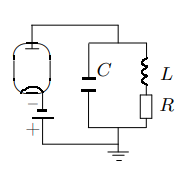
\includegraphics[width=0.8\linewidth]{установка}
	 	\caption{Схема подключения колебательного контура}
	 \end{wrapfigure}
	 
	 Для обнаружения дробового шума в анодную
	 цепь лампы включена нагрузка
	 — параллельный
	 колебательный
	 контур (рис. 1).
	 Токовый импульс, связанный с про
	 хождением электрона через диод, приводит
	 к зарядке конденсатора
	 C, который
	 входит в состав
	 контура LC
	 R. В
	 контуре возникают электрические
	 колебания. Следующие электроны
	 — в зависимости от фазы
	 колебаний
	 контура
	 —
	 усиливают или ослабляют
	 колебательный процесс. Постепенно
	 в контуре возбуждаются
	 колебания, амплитуда
	 и фаза
	 которых случайным образом меняются во времени. Кроме заряда, связанного с колебательным процессом, на
	 конденсаторе есть,
	 конечно, заряд, возникающий из-за наличия среднего тока. Этот заряд нас интересовать не будет.
	 Среднее значение амплитуды
	 колебаний
	 контура мо
	 жет быть найдено из
	 энергетических соображений.
	 Установившееся значение амплитуды определяется тем, что средняя энергия,
	 которую приносят электроны на
	 конденсатор, равна энергии,
	 которая рассеивается в колебательном
	 контуре.\\
	 Пусть при электрических
	 колебаниях в контуре мгновенное значение
	 напряжения на
	 конденсаторе равно
	 \begin{equation}
	 	U = U_0cos(\omega t)
	 \end{equation}
 	Тогда после пролета одного электрона заряд на конденсаторе станет равным:
 	\begin{equation}
 		q_2=q_1+e=CU_0cos(\omega t) + e
 	\end{equation}
 	Энергия конденсатора рассчитывается по формуле:
 	\begin{equation}
 		W = \frac{q^2}{2C}
 	\end{equation}
 	Тогда ее приращение после пролета электрона:
 	\begin{equation}
 		\Delta W = \frac{q_2^2 - q_1^2}{2C} = \frac{2CU_0cos(\omega t) + e^2}{2C}
 	\end{equation}
 	\begin{figure}[H]
 		\centering
 		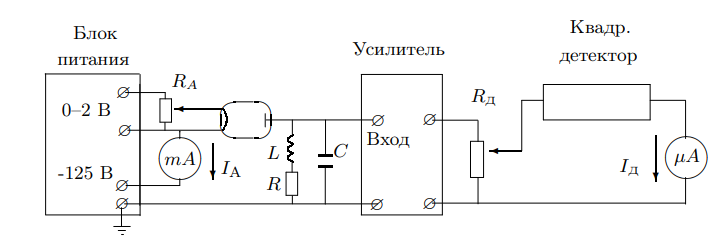
\includegraphics[width=0.9\linewidth]{шум}
 		\caption{Принципиальная схема в режиме измерения напряжения шума}
 		\label{fig:}
 	\end{figure}
 	\begin{figure}[H]
 		\centering
 		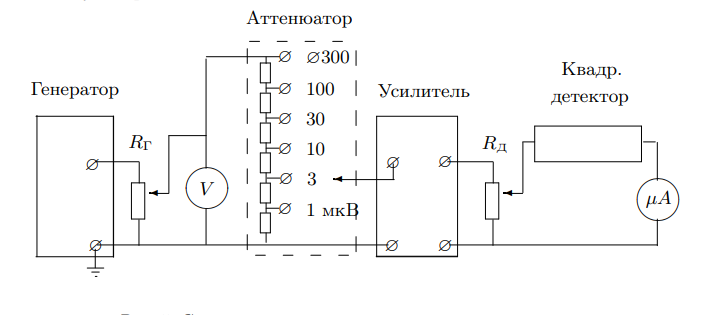
\includegraphics[width=0.9\linewidth]{доюротность}
 		\caption{Принципиальная схема в режиме измерения добротности}
 		\label{fig:}
 	\end{figure}
 	
 	Пусть в секунду через лампу про
 	ходят
 	N электронов. Полное увеличении
 	средней энергии
 	конденсатора складывается из
 	N слагаемых, определяемых формулой (4). При этом вклад от первого члена формулы обращается в нуль, так
 	как электроны приходят на
 	конденсатор в произвольные
 	моменты времени, а среднее значение $cos(\omega t)$ равно нулю. Средняя мощность, приносимая электронами на
 	конденсатор, определяется
 	только вторым слагаемым
 	и равна
	 \begin{equation}
	 	P = N \frac{e^2}{2C}
	 \end{equation}
 	Рассчитаем теперь потери в сопротивлении. Про
 	ходящий через него
 	ток $I_R$ складывается из постоянного тока $I_=$
 	и
 	колебательного тока
 	контура
 	$I_{\approx}$. Выделяемая в сопротивлении мощность в среднем равна
 	\begin{equation}
 		⟨P_R⟩=⟨I^2R⟩=R⟨(I_= + I_\approx)^2⟩
 	\end{equation}
 	где угловые скобки обозначают
 	усреднение по времени. Переменная составляющая тока может быть выражена через напряжение на
 	конденсаторе:
 	\begin{equation}
 		I_\approx = \frac{dq}{dt} = -CU_0sin(\omega t)
 	\end{equation}
 	Подставим (7) в (6), возведем сумму $I_=$ и $I_\approx$ в квадрат
 	и
 	усредним результат по времени. Замечая, что среднее значение $<sin(\omega t)> = 0$, а $<sin^2(\omega t)> = \frac{1}{2}$, найдём
 	\begin{equation}
 		⟨P_R⟩ = RI_=^2 + R⟨I_\approx^2⟩ = RI_=^2 + \frac{1}{2} R C^2 U_0^2 \omega^2
 	\end{equation}
 	Таким образом, мощность, выделяемая в сопротивлении
 	R, — это мощность,
 	которую выделяют в нём постоянный ток диода
 	и ток
 	колебаний,
 	возникающий в контуре из-за дробового шума.
 	Приравняем мощность (5), возбуждаемую электронами в контуре,
 	к мощности теряемой в сопротивлении из-за наличия
 	колебаний:
	 \begin{equation}
	 N \frac{e^2}{2C} = \frac{1}{2}R (CU_0\omega)^2
	 \end{equation}
 	Заметив, что
 	$Ne =
 	I_а$, а амплитудное значение напряжения на
 	конденсаторе
 	U0 связано с эффективным значением
 	$U_{эфф}$ обычным соотношением
 	$U^2_{эфф}
 	= \frac{U_0^2}{2}$, найдём для заряда электрона $e$ следующую формулу:
 	\begin{equation}
 		e = \frac{2 \omega^2C^3RU_{эфф}^2}{I_a}
 	\end{equation}
	 Таким образом, измеряя ток
	 $I_a$, проходящий через диод,
	 и среднеквадратичное напряжение шума на
	 контуре
	 $U^2_{эфф}$, можно определить заряд
	 электрона. Формула (10) может быть записана через добротность
	 контура. Как известно, добротность контура
	 $Q$ связана с его параметрами
	 формулой
	 \begin{equation}
	 Q = \frac{1}{\omega RC}
	 \end{equation}
	 Окончательная формула для расчёта заряда электрона имеет вид
	 \begin{equation}
	 	e = \frac{2 \omega C^2U_{эфф}^2}{I_a Q}
	 \end{equation}
 	\newpage
	\section{Ход работы}
	\subsection{Проверка квадратичности детектора}
	\subsection{Рассчет заряда электрона}
	Проведем измерение заряда электрона согласно техническому описанию работы.\\
	\begin{table}[H]
		\centering
		\begin{tabular}{|c|c|c|c|c|c|c|c|}
			\hline
			$I_a,~ мА$             & $I_д,~ усл.~ ед.$ & $U_{эфф},~мкВ$ &$U_{1},~мкВ$ & $\Delta I, ~усл.~ед.$ & $U_{2},~мкВ$ & $Q$     & $\sigma Q$ \\ \hline
			\multirow{5}{*}{1} & 72  & 78   & 0.32     & 12      & 60  & 187.5 & 4.3     \\ \cline{2-8} 
			& 40  & 75   & 0.4      & 17      & 66  & 165.0 & 4.8     \\ \cline{2-8} 
			& 48  & 74   & 0.5      & 36      & 86  & 172.0 & 4.0     \\ \cline{2-8} 
			& 60  & 75   & 0.46     & 40      & 82  & 178.3 & 4.4     \\ \cline{2-8} 
			& 80  & 76   & 0.25     & 18      & 47  & 188.0 & 4.4     \\ \hline
			\multirow{5}{*}{2} & 40  & 100  & 0.6      & 6       & 81  & 135.0 & 2.4     \\ \cline{2-8} 
			& 50  & 96   & 0.8      & 17      & 96  & 120.0 & 2.0     \\ \cline{2-8} 
			& 60  & 96   & 0.9      & 34      & 111 & 123.3 & 1.8     \\ \cline{2-8} 
			& 70  & 96   & 0.7      & 40      & 96  & 137.1 & 2.4     \\ \cline{2-8} 
			& 90  & 99   & 0.4      & 24      & 60  & 150.0 & 3.2     \\ \hline
			\multirow{5}{*}{3} & 40  & 114  & 0.96     & 7       & 105 & 109.4 & 1.5     \\ \cline{2-8} 
			& 50  & 114  & 0.94     & 4       & 96  & 102.1 & 1.5     \\ \cline{2-8} 
			& 70  & 114  & 0.8      & 28      & 96  & 120.0 & 2.0     \\ \cline{2-8} 
			& 78  & 117  & 0.84     & 36      & 99  & 117.9 & 1.8     \\ \cline{2-8} 
			& 90  & 117  & 0.5      & 22      & 66  & 132.0 & 1.8     \\ \hline
			\multirow{5}{*}{4} & 40  & 126  & 2.1      & 22      & 189 & 90.0  & 2.2     \\ \cline{2-8} 
			& 50  & 126  & 0.9      & 16      & 90  & 100.0 & 1.6     \\ \cline{2-8} 
			& 60  & 126  & 0.8      & 24      & 90  & 112.5 & 1.9     \\ \cline{2-8} 
			& 72  & 129  & 0.9      & 34      & 99  & 110.0 & 1.7     \\ \cline{2-8} 
			& 80  & 129  & 0.7      & 28      & 84  & 120.0 & 2.2     \\ \hline
		\end{tabular}
		\caption{Замер эффективного напряжения контура и добротности при различных значениях накального тока}
	\end{table}
	По полученным значениям проведем усреднение и получим значение заряда электрона.\\
	Для расчета заряда электрона будем использовать формулу (12), требуемую емкость и частоту контура запишем с установки: $C = 1200 ~пФ; f = 125~кГц$.\\
	\begin{table}[H]
		\centering
		\begin{tabular}{|c|c|c|c|c|c|}
			\hline
			$I_a,~ мА$ & $<Q>$ & $\sigma <Q>$& $<U_{эфф}>,~мкВ$  & $е \cdot 10^{-20}, ~Кл$   & $\sigma  е\cdot 10^{-20}, ~Кл$ \\ \hline
			1      & 178.2  & 4.6     & 75.6  & 7.3 & 0.8     \\ \hline
			2      & 133.1  & 2.7     & 97.4  & 8.1 & 1.1     \\ \hline
			3      & 116.3  & 1.9     & 115.2 & 8.6 & 0.9     \\ \hline
			4      & 106.5  & 2.1     & 127.2 & 8.6 & 1.0     \\ \hline
		\end{tabular}
		\caption{Рассчет заряда электрона по значению эффективного напряжения и добротности контура}
	\end{table}
	Итого получаем для заряда электрона значение: $e = (8.15\pm 1.1) \cdot 10^{-20}~Кл$.
	\newpage
	\section{Обсуждение результатов}
	\textbf{Табличное значение заряда электрона в СИ: $e = 1.6 \cdot 10^{-19}~Кл$\\
	Значение полученное в ходе эксперимента:  $e = (8.15\pm 1.1) \cdot 10^{-20}~Кл$\\}
	Полученное нами значение в 1.96 раза меньше табличного, при этом мы видим что значения замеренные при различных значениях накального тока не противоречат друг другу, что может косвенно говорить о верном ходе замеров.
	\subsection*{Возможные причины расхождения}
	1) Вероятными могут быть как плохой контакт и другие неисправности установки, однако перед выполнением работы исправность установки была проверена, а в ходе самой работы дополнительно проверили квадратичность детектора.\\
	2) В ходе вывода формул мы совершили одну важную оговорку (См. Введение жирный шрифт): мы предположили что лампа работает в режиме насыщения и в пространстве между электродов отсутствуют какие-либо заряды. Отсюда получили предположение что $Ne = I_a$, в нашем же случае сравнивая с табличным значение электрона получаем что за выбранный период пролетает только $\frac{N}{2}$ электронов.\\
	\subsection*{Закон "трех-вторых"}
	В работе исследуется зависимости прямого тока, проходящего через вакуумный диод, в зависимости от напряжения на нем, а именно та часть вольт-амперной характеристики, в которой электронное облако существенно влияет на распределение электрического поля между катодом и анодом.
	
	Распределение потенциала по радиусу внутри диода определяется уравнением Пуассона в цилиндрических координатах:
	
	\begin{equation}\label{}
		\Delta V = \dfrac{d^2V}{dr^2} + \dfrac{1}{r} + \dfrac{dV}{dr} = - \dfrac{\rho(r)}{\epsilon_0}
	\end{equation}
	
	При этом плотность заряда $ \rho(r) $ связана с текущим через слой диода толщины $ l $ током $ I $ формулой $ I = -2\pi r \rho(r)v(r)l$. При этом из закона сохранения энергии мы легко находим скорость $ v(r) $ электронов , прошедших через разность потенциалов $ V(r) $: $ \frac{mv^2}{2} = eV(r) $.  Отсюда мы получаем уравнение 
	
	\begin{equation}\label{ur}
		r \dfrac{d^2V}{dr^2} + \dfrac{dV}{dr} = \dfrac{I}{2\pi\epsilon_0}\sqrt{\dfrac{m}{2eV}}
	\end{equation}
	
	Однако, в дифференциальном уравнении 2-ого порядка относительно $ V(r) $ нам неизвестен ток I, зависящий от V. Для доопределения уравнения будем полагать:
	
	\begin{equation}\label{usl}
		\dfrac{dV}{dt}\bigg |_{r=r_k} = 0
	\end{equation} 
	
	Наше предположение означает что вблизи катода пространственный заряд электронов полностью экранирует поле анодной разности потенциалов.
	
	Уравнение \eqref{ur} является нелинейным. Попробуем  найти некое частное решение, где $ V_a = V_{a0}, $ при котором ток $ I = I_0 $. Тогда выражения 
	
	\begin{equation}\label{}
		I = I_o \left( \dfrac{V_a}{V{a0}} \right) ^{3/2}, \qquad V(r) = V_{a0}(r)\dfrac{V_a}{V_{a0}}
	\end{equation}
	
	являются решением уравнения \eqref{ur}, что проверяется подстановкой. В общем виде решение записывается в виде
	
	\begin{equation}\label{3/2}
		I = \dfrac{8\sqrt{2}\pi \epsilon_0 l}{9}\sqrt{\dfrac{e}{m}}\dfrac{1}{r_a\beta^2} V^{3/2}
	\end{equation}
	
	Это и есть так называемый "<закон трех вторых"> -- ток в вакуумном диоде пропорционален напряжению на нем в степени 3/2. Он справедлив при любой геометрии электродов, если ток не слишком велик (т.е. пока выполнено условие \eqref{usl}). 
	
	Так как нам нужно найти удельный заряд электрона, выпишем в явном виде его из уравнения \eqref{3/2}:
	
	\begin{equation}\label{e/m}
		\dfrac{e}{m} = \dfrac{81r_a^2\beta^4}{128\pi^2\epsilon_0^2l^2}  \dfrac{I^2}{V^2} = k  \dfrac{I^2}{V^3} = k (\frac{dI}{dV^{3/2}})^2
	\end{equation}
	
	Таким образом, удельный заряд электрона определяется из отношения квадрата тока к кубу напряжения, умноженный на коэффициент, зависящий от параметров установки.
	
\end{document}
